\subsection{Диаграмма прецедентов приложения}
\label{sec:design:algorithm}

Диаграмма прецедентов в UML диаграмма, отражающая отношения между актёрами и прецедентами и являющаяся составной частью модели прецедентов, позволяющей описать систему на концептуальном уровне.

Прецедент, также: вариант использования, сценарий использования — спецификация последовательностей действий (варианты последовательностей и ошибочные последовательности) в Унифицированном языке моделирования (UML), которые может осуществлять система, подсистема или класс, взаимодействуя с внешними действующими лицами.

Сформируем модель вариантов использования разрабатываемой системы (рисунок~\ref{sec:design:use_case}).

Основным актером, взаимодействующим с системой, является <<Пользователь>>, который взаимодействует с программным средством создания веб-приложений с помощью 
готовых графических компонентов. Данный пользователь, используя графический интерфейс данного программного средства, получает доступ к его функциям. В качестве пользователя может выступать как конечный пользователь приложения, в которое будет интегрироваться данное программное средство, или сам разработчик в процессе разработки своего программного средства.

Ограничение функциональности для пользователей могут определять разработчики, интегрирующие данный программный модуль свое программное средство. Да и потом, сами разработчики могут в процессе разработки пользоваться данным инструментом с целью ускорения процесса разработки путем автоматизации тривиальных действий создания графический компонентов.\pagebreak

На основании диаграммы прецедентов программного средства, изображенной на рисунке~\ref{sec:design:use_case} можно выделить следующие сценарии его использования:
\begin{itemize}
    \item применение пресета из списка доступных;
    \item очистить грид-разметку;
    \item отменить предыдущее действие;
    \item переключить текущий вид, используя меню;
    \item изменить размер сетки грид-разметки;
    \item применить компонент путем перетаскивания нужного из списка компонентов на грид-разметку;
    \item сохранить пресет;
    \item сгенерировать код приложения;
    \item выбрать компонент и применить в его отношении изменения.
\end{itemize}

\begin{figure}
\centering
    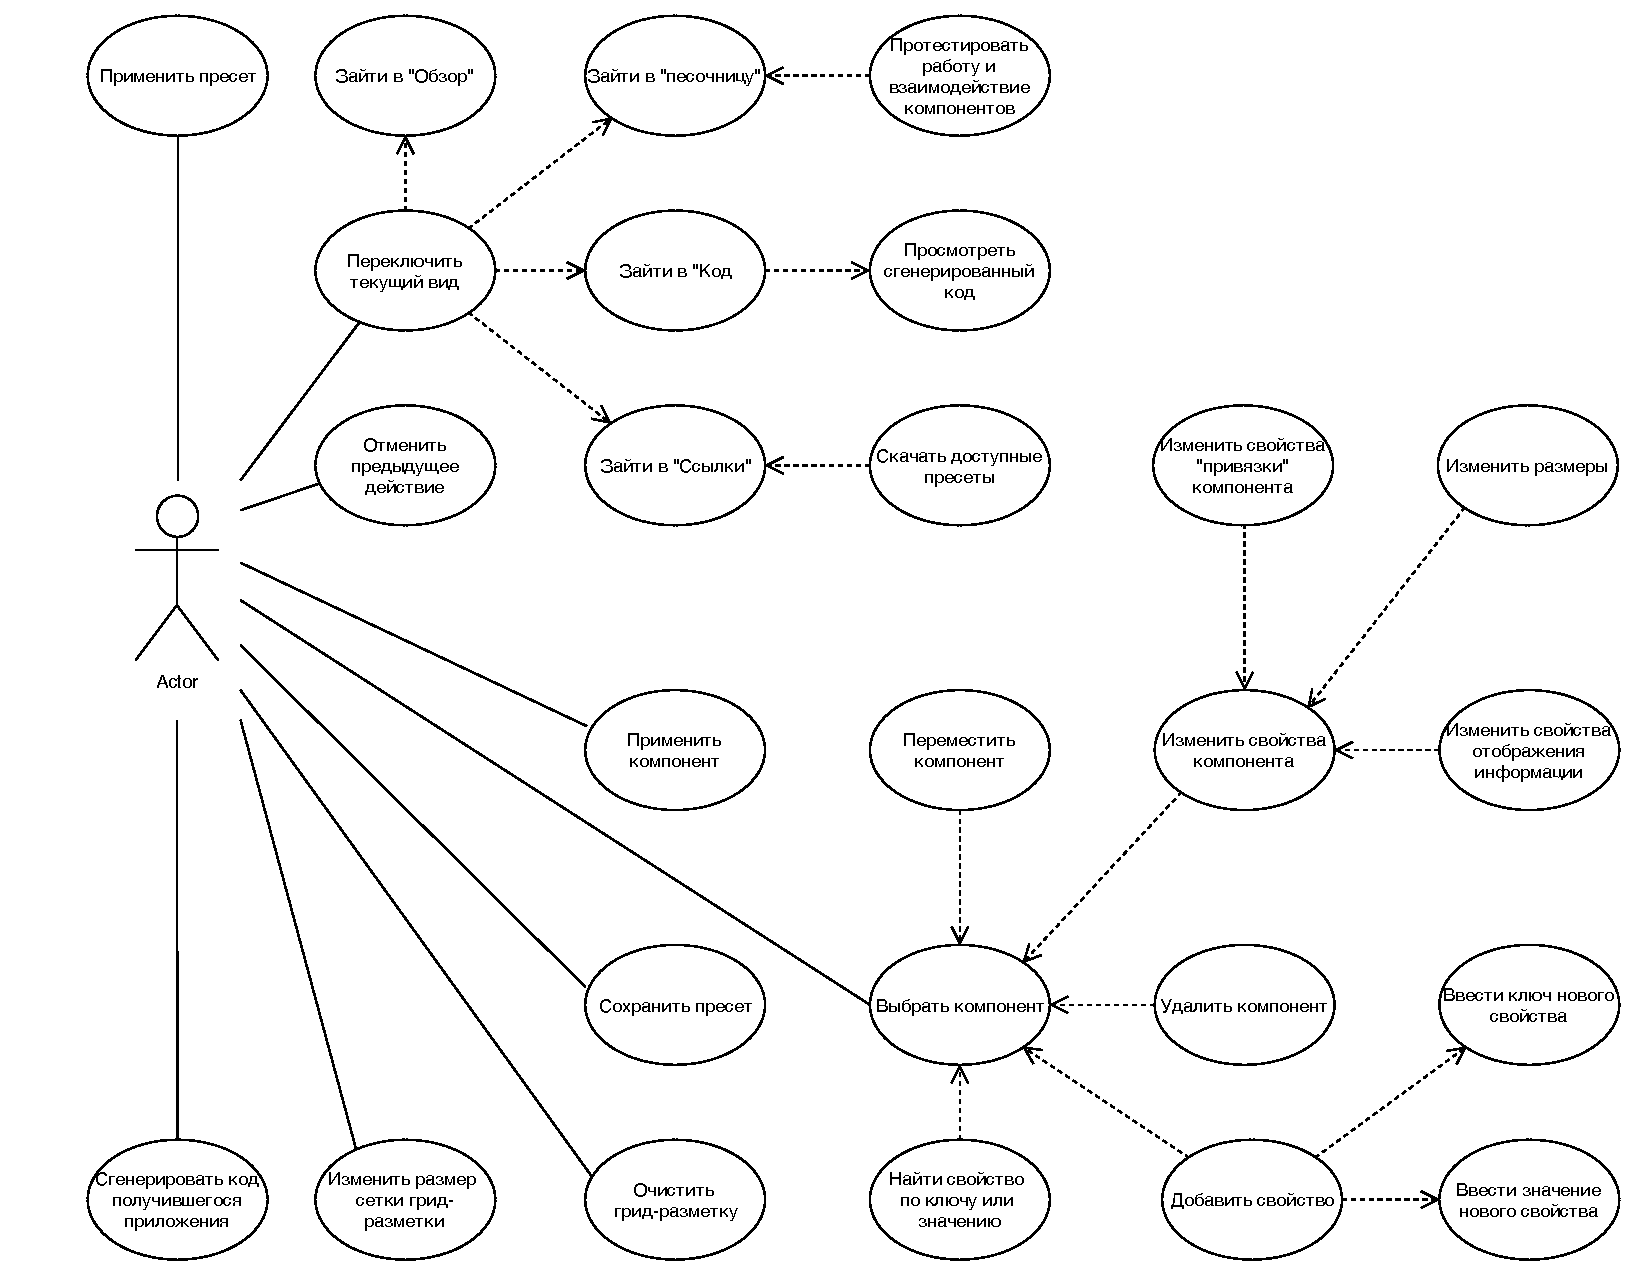
\includegraphics[scale=0.40]{Use_case.pdf}
    \caption{Диаграмма прецедентов приложения}
    \label{sec:design:use_case}
\end{figure}

Таким образом можно сделать вывод, что программное средство представляет собой довольно гибкий и многофункицональный инструмент. Однако определять доступность всей функциональности конечному пользователю будут разработчики, интегрирующие данное программное средство в свой продукт: ведь не каждому пользователю нужно настолько глубокая кастомизация приложения - большинству хватит просто расположить графические компоненты согласно собственным предпочтениям, не вдаваясь в подробности <<связывания>> компонентов.

Гибкость в определении доставляемой пользователю функциональности является большим преимуществом данного программного средства.

